\section {物料计划与控制}

\subsection {物料控制过程}
.
    \begin{center}
        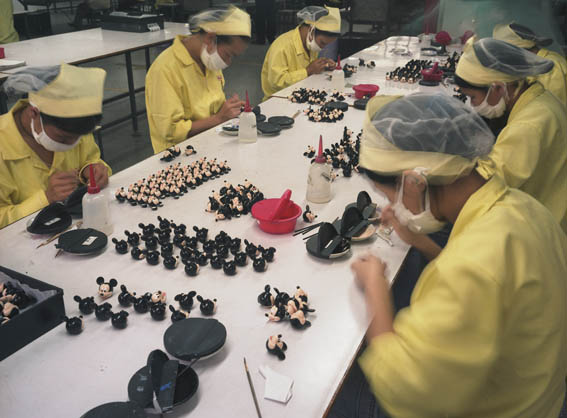
\includegraphics[scale=0.5]{pline1.jpg}
    \end{center}

    物料控制是为了控制好原料及其他物料的采购,不要出现近期生产不用却采购回大批物资积压在仓库,造成仓库库存太多,也不要出现马上该生产用原料了,而采购物资却仍不到位。最好是达到恰好要用恰好就到货,实现零库存或接近零库存的目的。

    物料控制的主要职能是物料计划、请购、物料调度、物料的控制(坏料控制和正常进出用料控制)等。物料控制通过制定行之有效的生产计划管理方案,使物料与生产管理工作顺畅,保证客户的需求,提高客户的满意度,同时提高生产效率,降低综合成本,进而提升公司的整体实力。

    对于接订单生产的企业。首先接到单后销售要把单传到物料控制员。并注明要求送货日期。物料控制员按排车间生产(有的是车间调度员安排,物料控制员只传单减库存)。按排生产的数量是单上要求到货数量加上动态库存数量减去仓库实际库存数量。生产部按照要生产的数量进行排程,并把排程结果交给物料控制员。物料控制员再计算该订单是否需要采购物料。采购物料到货日期就是生产订单前一天。

    物料控制的管理过程如下:

    职责分配:
        \begin{enumerate}
            \item  物料控制员对物料分析,使公司即不出现物料积压占压资金,又不出现停工待料。
            \item  市场部:负责订单下达及交期评审。
            \item  研发部:负责订单BOM制订及生产工艺设计。
            \item  PMC部:负责生产与物料计划的制订及协调跟进。
                \begin{enumerate}
                    \item  计划处:订单物料的发放、申购、跟踪及生产进度的跟踪。
                    \item  采购:负责物料的采购及跟进工作以及供应商评审。
                    \item  外发:负责物料的外发及进度跟进工作。
                    \item  货仓:负责物料进出仓控制及库存物料的质量控制。
                \end{enumerate}
            \item  生产部:负责生产前期准备工作及按计划完成生产任务,对生产进度及异常进行处理控制并反馈!
        \end{enumerate}

     \begin{enumerate}
        \item  交期评审:接订单后,市场部、研发部同PMC、生产部联合进行评审产品设计要求,货期,物料采购周期等,并出其《订单评审报告》。

        \item  编制生产计划:按评审的订单及时制订生产计划,包括生产进度计划,物料需求计划和设备要求计划。

            \begin{itemize}
                \item  生产计划
                    \begin{enumerate}
                        \item  对工厂设备人员,及生产能力进行分析评估,及香港上料之物料交期确认来制定具体生产计划。
                        \item  编制周生产计划,收集、汇总、縂计分析每日生产报表,根据生产进度异常,物料,技术,品质,工艺的变化,做生产计划调整。
                        \item  对生产进度落后,结合生产实际情况,同市场部沟通实际交期客人是否同意,再修正出货计划.
                    \end{enumerate}
                \item  物料控制:
                    \begin{enumerate}
                        \item  分解物料清单,根据仓库库存状况确定物料净需求量,根据经济订购量和生产计划,确定物料每次订购数量同交货期限,编制物料需求计划及订货计划。
                        \item  根据生产计划确认具体物料入库时间,协调采购,对可能缺料的订单重点跟踪处理因物料供应脱节、进度落后、生产提前、计划变更、订单变更而出现的物料问题。
                        \item  物料入仓后,开具《物料发放单》、生产据单到仓领料,物料发放应遵循先进先出,按单办理的原则。
                        \item  欠料和追料:根据每周的生产进度安排确认下周的物料缺料状况,对物料不能按期回厂和欠料情况,及时通知相关负责人跟进解决。并每3小时跟催一次,对物料不能回厂并影响生产的及时通知上司寻求共同解决.
                        \item  退料和补料:对生产所退仓物料进行分类标识并申请处理,对物料异常所产生的补料必须经上级签字后方能补数并留补料单备查。
                    \end{enumerate}
            \end{itemize}
        \item  货仓根据物料需求计划,查实仓储情况并及时反映给采购、计划、外发同时通知QC检查品质。
        \item  采购部根据物料需求计划订购所需物料并及时跟进物料回厂进度,做到适时供应生产物料。
        \item  外发根据物料需求计划同设备要求计划结合本厂实际情况时外发及跟进物料回厂进度。
        \item  生产根据生产进度计划进行编制作业组织生产,对各工序进度控制,异常调整,按时完成生产任务,成品经QA检验合格后填写,《成品入库单》,同仓库进行成品交接.
        \item  计划处出具出货计划表,合理间次安排装柜时间并通知香港船务部,仓库根据此安排入库工作并据香港船务部《收货通知单》安排装柜进行出库作业。
        \item  PMC每周出其货表共享,仓库及时填写《查货资料报告》并总结每月出货洭总。
    \end{enumerate}


\subsection {物料控制员}

    对制造业来说,实现ERP的计划与控制已大势所趋。然而,在企业管理人员当中,有一类人不仅压力最大,而且也充满了困惑。在新的变革到来时,尤其是传统的行业,企业的物料控制员要么是恐惧,要么是不知所措,为了不被信息时代所淘汰,他们孜孜不倦的求索:在信息化时代,我们应如何面对?

    物料需求计划的技法能产生一个实时的信息系统

    虽然物料需求计划MRP的技法能给我们带来一个实时的信息系统,并且产生恰当的信息,从而使物料控制员对信息采取行动。MRP的技法体现在如下几个方面。

    \begin{enumerate}
        \item  始终保持动态的供需平衡,是库存降低为最低点,而不缺料
        \item  可以自动的计算(现有库存+在订量+在检量-已分配量)
        \item  采购计划与生产计划自动算出,减少数据重复录入,减少人为的计算错误
        \item  主计划与生产计划与采购计划有效衔接
        \item  计划可重排性
        \item  计划可以反查
        \item  可以计算能力并能力分析
        \item  计划可以模拟
        \item  计划更实时,真实
        \item  对销售计划快速响应,提高准时发运率
        \item  提高团队精神(MRP牵涉到技术,库存,销售,生产等部门)
    \end{enumerate}

    那么,我们还需做什么呢?

\subsubsection {有效的物料控制员应该有一套工作程序来使工厂避免陷入困境。}

    一名成功的,有效的物料控制员应该提前告诉工厂经理即将来临的问题并推荐行动防止它们对客户服务或对工厂高效作业产生严重干扰。计划与控制的真正职能是为了使工厂避免陷入困境,从而管理工厂所需的信息而不只是处理为摆脱困境而要进行的日常活动。MRPII制造控制系统是一门处理信息的系统 ,它要求特定的活动要在特定的时间进行。 物料控制员像其它职能经理一样最好制订一张日程表把每天要求他们注意的事情列入表中并遵循这张表首先去做最重要的工作。没有一名经理能够去关心所有存在的问题,所以把问题排序并首先处理更重要的问题是极其重要的。

    由于物料控制员的成就将主要地依赖于信息系统的准确性与敏捷性,时常,某些最重要但是例行的活动(复审物料计划或提前期)是因为紧急中断的压力而被拖延的。有时要把后来表明的不良结果同其真正原因相联系是困难的。如列出一个检查清单会对正确地组织生产控制部门的活动有很大的帮助。物料控制员应该是定期地(至少每月一次)坐下来对下六个月里已知的与预期的问题作ABC分析,排出最大的问题并确保设计出活动来处理与防止这些问题。一个良好的习惯是每天准备一张今日按优先次序的活动表。

    物料控制员的工作计划(仅供参考)

    \begin{enumerate}
        \item  日程计划准备好
        \item  公布生产计划
        \item  修订生产计划
        \item  复审MRP输出表
        \item  查询缺货表
        \item  更新发出原料库存报告
        \item  完成"ABC"类存货复审
        \item  审计成品库存
        \item  活动与问题汇总
        \item  编制生产延误报告
        \item  编制外购组件延误报告
        \item  复审提前期
    \end{enumerate}

\subsubsection {物料控制员应主动的介入管理信息系统并成为协调者}

    计划与控制的主要职能是管理好一个信息系统。但是,必须强调的不是被动地去做。物料控制员在向管理层提出替代方案和这些方案的成本与结果的分析时应采取主动。在一个季节性销售的公司里,物料控制员应提出多种替代的生产计划以揭示如果完全用平准化生产,将额外地持有多少库存,如果按销售订单生产则将增加多大能力,人员将会有多少改变等等。物料控制员应估计这些不同计划的成本,推荐一份计划给管理层并协助做出基本的决策。一旦做出决策之后,物料控制员的工作就是控制信息使工厂保持在正常的轨道上。由于在过程中有许多计划的偏离,这就需要有不断的校正行动。 具有讽刺意味的是,生产线人员如果没有采取恰当的校正行动时,一个制造控制系统就难以被认为是成功的。实际上,仅仅产生了正确信息,这只是告诉经理们需要做什么而已。并不保证将采取的行动是正确的。往往物料控制员最容易受责难的原因是用其他人的行动来判断他的绩效。即使该系统指出需要增加能力而且这一增大能力的估计已经及早地通知了工厂作业人员或更高一级经理,但他们拖延不去增加,当结果使客户服务变差时,受埋怨的往往是计划与控制小组或物料控制员。几乎每个人都知道客户服务不好,但很少有人能识别出其真正原因。在ERP的管理信息运行的同时,物料控制员们经过有效的培训应该能采取行动。如果他们内行地做他们的处理信息的工作,他们将使所有有关人员知道需要采取什么行动并且谁要负责去采取这些行动。

    制造控制系统所生成的信息往往把巨大的压力施加在物料控制员的肩上,甚至加在往往是物料控制员上司的制造经理肩上。如果物料控制员对系统没有信心,如果他们不采取主动并且强有力地与勇敢地提出问题,他们会成为代人受过的“好人”,因别人不能采取恰当行动而自己受埋怨。制造控制系统必须能经得起来自物料控制员们的相当大的压力与挑战,他们总是对该系统产生的信息表示怀疑并要求作彻底的复审或进一步分析导致来推迟采取行动。能被证实的或能被容忍的怀疑态度的重要性应该有一个限度。在这一点上,能干的物料控制员应该得到其上司的强有利的支持以克服消极的阻力并采取有效的行动而不再进一步要求该系统证明它自己是可靠的。保持主动和进取心,再配上良好的系统与胜任的操作人员。每天,物料控制员们及其办事人员必须做出关于未来的成百甚至上千个决定。事后看来不可避免有些决定是错的,批评者很容易指出在计划过程中所犯的错误。所以物料控制员必须与其他经理们协调其工作目标为整个企业的目标。以避免在强调责任制的组织里会出现部门壁垒和信息孤岛现象。 物料控制员应承认救火是必要的,但防火才是更重要的。

    救火是必要的,但防火才是更重要的。制造控制中最严重的引诱之一就是去当一名救火员:每天早上一上班就准备接电话,然后马上冲出去。这毫无疑问地满足着那些强调行动的人,给人觉得非常有能力和可以把手指按在工厂脉搏上并随时知道什么事情正在进行中的经理的形象。不幸的是,这种救火活动在现实中是经常发生,但也是不可缺少的。导致防火的意识容易被忽视。如找出主要机床的寿命,弄清它们是否及时更新以达到所需能力或分析建议是否添置新产品的设备。何时,何处可能发生瓶颈,如何避免它们,这些工作看来确实是平凡的而不像救火一样轰轰烈烈。 忽视防火的物料控制员可以肯定明天将带来更大更好的救火机会。物料控制员必须对麻烦有思想准备。墨菲定律是“可能出错的问题,往往就在最不适宜的时间出现”就是在工厂里发明的。物料控制员应该是快乐的悲观者,他承认问题是一种生活方式,明天的问题今天毫无疑问正在酝酿着。工厂里的危机很少是一夜之间造成的,它们通常在一个长时期的酝酿而且时常是久久未采取行动的结果。物料控制员有责任及早指出麻烦可能出现何处,指出有哪些办法并做一切可能做的事去确保作业按计划持续进行或被校正以防止出现危机。 物料控制员必须在及时采取行动和未来准备改善计划之间取得平衡

    有效的控制信息的最主要特征之一就是它的及时性。是事后给出辩解还是及早地提出信息使得有人能采取措施去防止问题。如果物料控制员的上司询问为什么一种产品缺货了,而经过一些调查,他被告知它是由上周电镀部门一个瓶颈引起的,该物料控制员只是给出了一种辩解。如果,另一方面,该物料控制员早就曾指出该瓶颈并提出正面建议去克服它而且预言如果这个瓶颈不解决产品将会缺货,那么他就是发出了一个控制信息。这简单的差别就在于及时性,向工厂作业人员及时提供信息使他们在麻烦发生之前去采取必要的校正行动。

    为保持有效的运作,物料控制员必须用客观的,建设性的方式去使用他们的信息与知识的力量。他们应该是现实主义者,并避免乐观主义的痴心妄想,去指望麻烦可能不会发生或如果你不理它它就会自己跑掉。他们必需经常在提醒人们注意现存的与潜在的问题,可是,他们必须避免责备或说别人不能胜任并且不要忍不住去证明自己永远是正确的。

    物料控制员每天应抽出一些时间去访问工厂里主要的或关键的生产区域。往往快速地在工厂里兜一趟将发现潜在的问题比最最及时更新的信息系统还快得多。物料经理还必须抽出一点时间,这多半需要在工厂正规上班时间以外,去思考与计划对本部门未来绩效至关重要的事。这是他想出防火项目与改善本部门绩效的长期计划的时候。一名优秀的物料控制员应努力使解决今天问题的行动与防止明天问题的计划之间达到平衡。虽然其办公室的力量在解决许多日常危机中是需要的,但他们必须避免过多地直接介入于催稽之中。必须有一个为未来做准备的计划去平衡这种工作。

\subsubsection {物料控制员必须接受计划控制的教育与培训}

    为未来做准备最重要步骤之一就是培训。必须包括新技法、新系统、更现代化的设备的开发与使用的教育,以及通过参与专业机构去扩大眼界与听专门的课程以获得制造控制领域或其他企业管理领域的知识。这个教育还应包括厂内计划。我们大部分的生产管理人员开始从事计划与控制工作时并未在此领域中学习过。他们不仅对生产控制知识知之不多,而且往往并不理解有许多东西要学。这类人往往变成催稽员与救火人员而并无多大能力去有效地控制生产。实际上,现在该领域已成为具有独特知识主体、术语、技法与应用的一门真正的专业。目前,在国内,还没有一个专门的机构来认证合格的专业人员。如在财务领域,我们已有CPA资格考试,等等。而在国外,可以通过APICS参加考试,由此可被证明作为技术上合格的专业人员。

    目前,国内ERP培训,和各个软件功能培训比比皆是,而缺少像APICS这种机构,对专门从事生产控制人员的资格培训。我们在大力推广信息化的同时,往往忽视了基础的工作。 实际上,这种教育由于其对象主要是成年人,所以,尽可能切合实际。如果人们能具体地看到每种技法如何应用到他们的公司,或看到曾经在过去引起过的问题,他们会热烈地做出响应。每个人都有希望对自己的工作更加精通。然而,需要接受有关制造控制活动的教育培训的人远远超过计划与控制人员。公司里其它部门经常把计划控制小组当作替罪羊,对所产生的任何信息表示怀疑从而减少他们根据这一信息采取行动的需要。让这些部门主管懂得一个制造控制系统是什么,他们必须如何同它合作并使用它,他们提供的信息与他们所采取的行动会如何对系统的绩效产生影响,这是任何公司的成功所不可缺少的。 最高层管理人员往往对制造控制系统的真正作用也知之不多。他们不知道在库存与生产管理方面有效的替代方案是有限的而且并不总是意识到有必要去平衡日常作业中互相冲突的目标。一项广泛的教育培训计划,最起码可以让一部分人认识到从计划与控制活动可以期望什么与不可以期望什么。

    归根到底,一个乐于冒险去设定有雄心的目标的物料控制员,一个努力工作去改善部门的作业并在实施MRP生产与库存控制的经理、一个想提高客户服务水平,改善工厂整体绩效的经理,将不难说服管理层相信他的工作的重要性与价值。

\subsubsection {物料控制员必须降低库存}

    库存过多且伴以许多缺货已成为常规而非例外。而且可能还会持续一段时间,导致库存的原因有:

    \begin{enumerate}
        \item  不准确的预测与不可靠的供应,要求成品超过预期的需求。
        \item  不可靠的供应商与长而不确定的采购时间,使得过量的原料与外购组件成为必要。
        \item  经常的调整,不稳定的物流,不良的质量,报废与返工,不完善的机床安装与设备,使得大量的在制品成为必要。
        \item  种种变化引起报废的库存。
    \end{enumerate}

    现代的方法拒绝接受这些作为不可避免的条件。干扰计划作业的一切问题可以而且必须解决。管理层不断施加压力去减少库存是对的。事实证明,在任何公司里“正确的”库存量比现存于许多企业中的要少而比现存于大多数企业中的要少得多。正当的步骤如下:
    \begin{enumerate}
        \item  设定一个要在规定期间(例如6个月内)减少(譬如25%)的挑战性目标。
        \item  提出投入(外购物料与生产工时)与产出(发货)速率指标并每月监控它们。迅速而敢做敢为地去校正偏差。
        \item  使减少库存的目标成为公司范围的计划,各个部门都有角色要担当。只有通过找出并解决过剩的原因才能显著地削减库存。
    \end{enumerate}

\subsubsection {物料控制员必须缩短提前期}

    没有比缩短越提前期更重要的工作了。这种观点同制造作业中许多人所持的观点相反;他们都需要更多时间来确保更好的绩效。他们的经验通常支持这种信念:缺货需更长时间去克服,过多的负荷要用更多时间去处理,而延误是时间不够的证明。

    实际上,削减提前期已被证明是可能的,较容易的而且最为有效的。一项有效的措施是:

    \begin{enumerate}
        \item  用厂外与厂内课程进行教育培训
        \item  选择一个具有长而不稳定的提前期并供应着大量产品的供应商
        \item  选择具有大量订单积压的工作中心
        \item  选择不稳定负荷与太多的在制品的工序
        \item  设计更短的调整或换装
        \item  实施投入/产出控制
        \item  使物料保持流动,缩小批量
        \item  顶住非难,坚持信念
    \end{enumerate}

\subsubsection {生产计划与控制的未来}

    制造控制原先是一种文书工作职能:维护库存与订单记录,发放车间订单与处理其它必要的记录保管职能。从那里它发展到包括存货催促与一些部门的机器负荷计划──但大多数技法是粗糙的而功能高度分散,直到许多公司把库存控制从生产控制分离出来。导致每个小组倾向去考虑它自身的有限目标而不是公司的总体目标。这一朝着分散化的倾向使控制问题复杂化,因为它使得要让财务、制造与销售经理们朝着共同目标一道工作的任务更加困难了。

    1960年代里,实际工作者寻找安全存货的正确数量以便在针对需求中的变化与供应中的不确定性去缓冲作业。他们为有统计技法去更新预测与重新评价所需的缓冲库存量而感到高兴。1970年代,人们弄清了即使需求有变化的有效的日程计划也是可能的,而且可以使用及时更新的优先级去改变补货提前期使急需的物品准时。强有力的MRP技法使这成为可能并在实际运用中得以普及。

    在二十世纪七十年代这10年里,所有需要的技法都开发出来并经过了试验。在二十世纪八十年代初,人们弄清了在最复杂的系统中所有的技法在大多数制造工厂的混乱环境里实际上是无能为力的。人们认识到了对缩短提前期有迫切的需要,并在成功的公司里开始认真地去减少记录误差,提高质量、缩小批量并理顺工厂里的物流。

    在2000时代,随着MRP的普及,工厂的混乱环境已得到改善,又随着计算机技术的发展,利用信息化的技术来提高解决企业效率的基本问题-能力约束。用FCS有限能力计划系统和扩展TOC的原理,全面进行多重资源约束的优化计划技法已出现。当然,仅仅能力约束还是不够的,还要考虑物料的约束、需求的约束,供应商资源约束、运输资源的约束、分销资源的约束、财务资金的约束,这就是APS高级计划排程系统的作用。还有些技法同时把JIT和TOC的优势结合在一起,形成了DFM需求流制造系统。在这信息高度发达的时代,企业的竞争是供应链的竞争,整合企业上游下游的供应链,使之形成供应链联盟,降低整个供应链的库存,缩短整个供应链的提前期,快速响应客户的需求。

    传统的组织形式将继续激烈地改变,去管理一个面临激烈竞争的制造企业所需的基本信息对每个公司来说将变得越来越不可缺少。计划与控制功能不仅在公司的业务中将变得更加重要,而且将成为高层管理人员不可缺少的培训领域。最高层经理必须学会如何去经营制造公司。

    对这些事实日益增长的意识,加上强烈的竞争,使人们更加重视计划工作,更加一体化的ERP系统使得计划的执行更加有效。制造业作为真正财富创造者的重要性给物料控制员们身上加重了一付责任的重担,要求他们用这个知识为公司,为国家而且也为他们自己谋取最大的利益。
